\documentclass[10pt,journal,compsoc]{IEEEtran}
%
% If IEEEtran.cls has not been installed into the LaTeX system files,
% manually specify the path to it like:
% \documentclass[10pt,journal,compsoc]{../sty/IEEEtran}

% Some very useful LaTeX packages include:
% (uncomment the ones you want to load)


% *** CITATION PACKAGES ***
%
\ifCLASSOPTIONcompsoc
  % IEEE Computer Society needs nocompress option
  % requires cite.sty v4.0 or later (November 2003)
  \usepackage[nocompress]{cite}
\else
  % normal IEEE
  \usepackage{cite}
\fi





% *** GRAPHICS RELATED PACKAGES ***
%
\ifCLASSINFOpdf
  \usepackage[pdftex]{graphicx}
  % declare the path(s) where your graphic files are
  % \graphicspath{{../pdf/}{../jpeg/}}
  % and their extensions so you won't have to specify these with
  % every instance of \includegraphics
  % \DeclareGraphicsExtensions{.pdf,.jpeg,.png}
\else
  % or other class option (dvipsone, dvipdf, if not using dvips). graphicx
  % will default to the driver specified in the system graphics.cfg if no
  % driver is specified.
  \usepackage[dvips]{graphicx}
  % declare the path(s) where your graphic files are
  % \graphicspath{{../eps/}}
  % and their extensions so you won't have to specify these with
  % every instance of \includegraphics
  % \DeclareGraphicsExtensions{.eps}
\fi

% My packages:
\usepackage{booktabs}
\usepackage{threeparttable}
\usepackage{cite}
\usepackage{hyperref}

% correct bad hyphenation here
\hyphenation{op-tical net-works semi-conduc-tor}


% Personal includes:
\usepackage{amssymb}
\usepackage{array}
\usepackage{amsmath}
\usepackage{breqn}

%%RK: My custom commands:
\newcommand{\norm}[1]{\left\lVert#1\right\rVert}
\newcommand{\ce}[1]{equation (\ref{#1})}
\newcommand{\cf}[1]{Figure \ref{#1}}
\newcommand{\cs}[1]{Section \ref{#1}}
\newcommand{\sip}[1]{\si[per-mode=symbol]{#1}}
\newcommand{\zero}{\mathcal{O}}
\newcommand{\pd}[2]{\frac{\partial #1}{\partial #2}}
\newcommand{\reals}{{\rm I\!R}}
\newcommand{\matrices}[2]{{\mathcal{M}(\reals)_{#1\times#2}}}
\newcommand{\naturals}{{\rm I\!N}}
\newcommand{\vecdisp}[3]{ \begin{bmatrix} #1\\#2\\#3\end{bmatrix}}

\begin{document}
%
% paper title
% Titles are generally capitalized except for words such as a, an, and, as,
% at, but, by, for, in, nor, of, on, or, the, to and up, which are usually
% not capitalized unless they are the first or last word of the title.
% Linebreaks \\ can be used within to get better formatting as desired.
% Do not put math or special symbols in the title.
\title{On the Backpropagation Method for Training Multi-Layer Perceptron Networks}

\author{Rian~Koja, \it{riankoja@gmail.com}}



% The paper headers
\markboth{CAP-351-3 Neurocomputing - Assignment Report}%
{Shell \MakeLowercase{\textit{et al.}}: On Methods for Training Multi-Layer Perceptron Networks}


\IEEEtitleabstractindextext{%
\begin{abstract}	
This report reviews some mathematical methods and tools associated with the Backpropagation Algorithm and with the numerical solution of nonlinear systems of equations. The Backpropagation algorithm is commonly employed for training neural networks. Their mathematical foundation is reviewed, and some considerations are given as to the implementation used by the Backpropagation algorithm.
\end{abstract}

% Note that keywords are not normally used for peer review papers.
\begin{IEEEkeywords}
Artificial Intelligence, Machine Learning, Multi-Layer Perceptron Classifier.
\end{IEEEkeywords}}


% make the title area
\maketitle


% To allow for easy dual compilation without having to reenter the
% abstract/keywords data, the \IEEEtitleabstractindextext text will
% not be used in maketitle, but will appear (i.e., to be "transported")
% here as \IEEEdisplaynontitleabstractindextext when the compsoc 
% or transmag modes are not selected <OR> if conference mode is selected 
% - because all conference papers position the abstract like regular
% papers do.
\IEEEdisplaynontitleabstractindextext
% \IEEEdisplaynontitleabstractindextext has no effect when using
% compsoc or transmag under a non-conference mode.



% For peer review papers, you can put extra information on the cover
% page as needed:
% \ifCLASSOPTIONpeerreview
% \begin{center} \bfseries EDICS Category: 3-BBND \end{center}
% \fi
%
% For peerreview papers, this IEEEtran command inserts a page break and
% creates the second title. It will be ignored for other modes.
\IEEEpeerreviewmaketitle



\IEEEraisesectionheading{\section{Introduction}\label{sec:introduction}}

\IEEEPARstart{M}{ethods} for training neural networks involve some process that updates the set of weights and biases that define each neuron that composes a neural network, as will be described in the following sections. Of particular interest, is the Back-propagation algorithm, which is based on gradient methods for optimizing nonlinear systems of equations. It consists of an iterative numerical algorithm that attempts to find a local minimum to an optimization problem and hopefully obtain an acceptable solution for the classification, regression, encoding, or similar problem that the neural network attempts to solve.

However, it can be shown that this problem can be treated as either under or over-determined depending on how it is spliced into smaller pieces and how it is approached. Either way, it inherits some of the shortcomings of the Newton-Raphson method that it implements. To show this, a review on these classes on methods is shown on \cs{sec:mathtools}, then some definitions are revisited in \cs{sec:nndef}, and finally the Backpropagation algorithm is reconstructed in \cs{sec:optimizing}

Some of the notation is inspired by \cite{haykin2010neural}, and some is derived from the literature of numerical methods, such as \cite{carnahan1969applied} and \cite{press1988numerical}.

\section{Mathematical Tools and Definitions}\label{sec:mathtools}

In this section, a few of the relevant concepts are recalled to lay the foundation required for the statements of the problems to be addressed and the approaches commonly found in the literature in similar contexts.

\section{Spectral Norm of a Matrix}
The spectral norm of a matrix $A$ is defined as the largest eigenvalue of the matrix $A$, it can be expressed as:
\begin{equation}
	\norm{A} = \max_x \frac{\norm{Ax}}{\norm{x}}
\end{equation}

\section{Frobenius Norm of a Matrix}
The Frobenius norm of a matrix $A$ is defined as the sum of the absolute values of the elements of the matrix $A$ squared. It can be expressed as:
\begin{equation}
		\norm{A} = \sqrt{\sum_{i,j=1}^n |A_{i,j}|^2} = \sqrt{\text{Tr}\left(A^TA\right)}
\end{equation}

\subsection{Lipschitz Functions}

A function $f:\reals^n \rightarrow \reals^m$ is said to be Lipschitzian if there exists $q>0$ such that:

\begin{equation}
\norm{ f(x) - f(y) } \leq q \norm{x - y} \, \forall x,y \in \reals^n 
\end{equation}

Where $\norm{ . }$ denotes the Euclidean vector norm, 

If a function is Lipschitzian, or a Lipschitz function then it is uniformly continuous and differentiable and its Jacobian $J\left[ f(x)\right]$ has a bounded spectral norm given by the same parameter $q$:
\begin{dmath}
{\norm{ f(x) - f(y) } \leq q \norm{ x - y } \, \forall x,y \in \reals^n }\iff {\norm {J\left[ f(x)\right] } \leq q \, \forall x \in \reals^n }
\end{dmath}

Here the spectral norm employed for the Jacobian is also denoted with $\norm{ . }$, though this is commonly indicated as $\left| . \right|_2$. Notably, this norm is smaller than or equal to the Frobenius norm of the same matrix, which in turn is much easier to compute.

\subsection{Moore-Penrose Pseudoinverse}

The Moore-Penrose pseudoinverse of a matrix $A$ is defined as:
\begin{equation}
	A^{\dagger} = \text{pinv}(A)
\end{equation}
It is defined by the following conditions:

\begin{itemize}
\item $AA^{\dagger}A = A$
\item $A^{\dagger}AA^{\dagger} = A^{\dagger}$
\item $\left(A^{\dagger}A\right)^* = \left(A^{\dagger}A\right)$
\item $\left(AA^{\dagger}\right) = A^{\dagger} A$
\end{itemize}

As from these definitions, the following properties arise:

When $A$ has linearly independent rows (full rank), the pseudoinverse can be computed as:
\begin{equation}
	A^{\dagger} = \text{inv}(A^T A) A^T
\end{equation}

Multiplying $A$ by a scalar $\alpha$ is equivalent to multiplying $A^{\dagger}$ by $\alpha^{-1}$:
\begin{equation}
	\left(\alpha A\right) ^{\dagger} = \alpha^{-1} A^{\dagger}
\end{equation}

If $A$ is invertible, then $A^{\dagger}=A^{-1}$.

\subsection{The Chain Rule for Multivariate Functions}
For a composition of scalar functions $f, g:\reals \rightarrow \reals$ one has:

\begin{equation}
	\frac{d (f \circ g)}{d x} = \frac{d f}{d g} \frac{d g}{d x}
\end{equation}

For multivariate functions $f :\reals^n \rightarrow \reals ^m$ and $g: \reals^m \rightarrow \reals ^p$, one might denote the chain rule as:
\begin{equation}
	J[f \circ g](x) = J[f](g(x)) J[g](x)
\end{equation}

If $A$ has a zero row, then $A^{\dagger}A$ has a zero column.


\subsection{Solving or Optimizing Nonlinear Systems of Equations}\label{sec:methods}

	Let:
\begin{equation}
	f:\mathbb{R}^n\rightarrow\mathbb{R}^m
\end{equation}
A system of (simultaneous) equations is given by:
\begin{equation}
	f(x)=\emptyset
\end{equation}

	Note that, for systems on a real domain:
\begin{equation}
	f(x^*)=\emptyset \Longleftrightarrow f^T(x^*)f(x^*)=0
\end{equation} 

Hence solving a system of equations effectively means solving one equation for several variables. Furthermore, because the product $f^T(x)f(x)$ is always positive, even if a solution does not exist, one may use similar methods employed for solving a system with the goal of minimizing a cost function expressed in this form.  However:
\begin{equation}
	\nabla\left[ f^T(x)f(x)\right]  = 2J\left[ f(x)\right] f(x)
\end{equation}

So at $x = x^*$ this expression evaluates to the null vector:
\begin{equation}
	\nabla\left[ f^T(x^*)f(x^*)\right]  = 2J\left[ f(x^*)\right] f(x^*) = 2J\left[ f(x^*)\right] \emptyset = \emptyset
\end{equation}

It may happen that for a given system there exists an inverse function $g(y)=f^{-1}(y)$ such that:
\begin{equation}
	g(\emptyset)=x^*\Longleftrightarrow f(x^*)=\emptyset
\end{equation}	

In general, this is an extremely fortunate situation, and no universal or sufficiently general method currently exists to construct one such function $f^{-1}(y)$ given only the expression or algorithm for $f(x)$. 

However, some standard methods are known in the literature for the case when the function $f$ has a known (and computable) derivative, the gradient-based ones being based on the original Newton-Raphson algorithm, which can be expanded for non-single variable equations in the following subsections.

\subsubsection{Square System Case}\label{sec:square}

Assuming $f:\reals^n\rightarrow\reals^n$, thus a square system of equations (same number of unknown variables and equations), for which a Jacobian matrix can be computed:
\begin{equation}
	J[f](x) = {\pd{f_i}{x_j}}(x)
\end{equation}

	Noting that if a Taylor Series for $f$ centered at $x_k$ converges for all points inside the disk $\norm{x^*-x_k}^2<R$, then:
\begin{equation} \label{eq:TaylorExpSol}
	f(x^*) = \emptyset = f(x_k)+J[f](x_k)(x^*-x_k)+\zero(\norm{x^*-x_k}^2) 
\end{equation} 

	Therefore:
\begin{equation}
	x^* = x_k - \left(J[f](x_k) \right)^{-1} f(x_k)+\left(J[f](x_k) \right)^{-1}\zero(\norm{x^*-x_k}^2) 
\end{equation}

	Newton-Raphson iteration function is given by:
\begin{equation}
	h(x) = x - \left( J[f](x) \right) ^{-1} f(x)
\end{equation}
Which in sequence notion yields:
\begin{equation}
	x_{k+1} = x_k - \left( J[f](x_k) \right) ^{-1} f(x_k)
\end{equation}
	Kantorovich’s theorem \cite{ortega1968newton} provides conditions for the convergence of such methods. But, in a simpler approach, for Lipschitzian $f$:
\begin{dmath}
	\norm{x_{k+1}-x_k}=\norm{\left(J[f](x_k)\right)^{-1}f(x_k)}\leq {\norm{\left(J[f](x_k)\right)^{-1}}\norm{f(x_k)}}\leq q^{-1}\norm{f(x_k)}
\end{dmath}

Therefore:
\begin{equation}
	\norm{x_{k+1}-x_k} = \leq q^{-1} \norm{f(x_k)}
\end{equation}

While:
\begin{dmath}
	\norm{f(x_{k+1})} = \left(J[f](x_k) \right)^{-1}\zero(\norm{x^*-x_k}^2) \leq q^{-1} \zero(\norm{x^*-x_k}^2)
\end{dmath}

Therefore:
\begin{equation}
	\norm{x_{k+1}-x_k} = \leq q^{-2} \zero(\norm{x^*-x_k}^2)
\end{equation}

So the method will converge quadratically if for each $x_k$ one has $q<1$. This assumes a small initial error, hence the method is sensitive to initial condition, and large derivatives may slow convergence since there would be a small norm for the inverse Jacobian. Problems arise with singular (or zero) derivatives. Two approaches are helpful:
\begin{itemize}
	\item Use Moore-Penrose Pseudoinverse for inverting the Jacobian.
	\item Multiply the inverse Jacobian by $\alpha$ with $0<\alpha<1$.
\end{itemize}

In machine learning, the scalar $\alpha$ is sometimes referred as the learning rate when performing a similar role.


\subsubsection{Underdetermined Case}\label{sec:undetermined}
If however, $f$ is a scalar field, that is $f: \reals^n \rightarrow \reals$, then instead of a Jacobian, it will have a gradient $\nabla f(x)$, and the Taylor Series developed in \ce{eq:TaylorExpSol}
\begin{equation}\label{eq:TaylorGrad}
		f(x^*) = \emptyset = f(x_k)+\nabla f(x_k)(x^*-x_k)+\zero(\norm{x^*-x_k}^2)
\end{equation}

This equation is approached as a linear system $b = Av$ with $b = f(x^*)-f(x_k)$, $A=\nabla f(x_k)$ and $v =x^*-x_k $, but since it has a one-dimensional equation over $n>1$ variables, the system is undetermined.  However, there exists a single solution to the optimization problem of minimizing $\norm{v}$ under the constraint that $b = Av$, which is given by $A^\dagger b$, where $A^\dagger$ is the Moore-Penrose pseudo-inverse of the matrix $A$, which for a vector simply corresponds to its transposed matrix with either the reciprocals of the non-zero entries and zero otherwise divided by the square norm of $A$. That is:

\begin{equation}
	A=\vecdisp{a}{b}{0} \Rightarrow A^\dagger = \frac{1}{a^2+b^2} \left[{a^{-1}},{b^{-1}},{0}\right]
\end{equation}


\subsubsection{Overdetermined Case}\label{sec:overdetermined}
Considering now a vector function on a scalar variable, that is: $f: \reals \rightarrow \reals^n$, such that instead of a gradient or a Jacobian, it actually has a derivative: 
\begin{equation}
	f(x^*) = 0 = f(x_k)+ \left. \frac{df(x)}{dx}\right|_{x=x_k}^T (x^*-x_k)+\zero(\norm{x^*-x_k}^2) 
\end{equation}

This equation is approached as a linear system $b = Av$ with $b = f(x^*)-f(x_k)$, $A=df(x)/dx|_{x=x_k}$ and $v =x^*-x_k $, but since it has a n-dimensional equation over a scalar variable, the system is over-determined. However, there exists a single solution to the optimization problem of minimizing $\norm{v}$ subject to the constraint $b = Av$, which can be discovered applying the method of Lagrange's multipliers.

Defining the Lagrangian as:
\begin{equation}
	L = \frac{1}{2} v^Tv + \lambda (Av-b)
\end{equation} 

Thus:
\begin{equation}
	\pd{L}{v} = v + \lambda A^T = \emptyset
\end{equation} 
\begin{equation}
	\therefore v = - \lambda A^T 
\end{equation} 

Since $\lambda$ is a scalar, one may already conclude that vector $v$ that solves the optimization problem has the same direction as the matrix $A$ (which corresponds to the derivative of the function $f$ originally). Recalling the constraint:

\begin{equation}
	Av-b = 0 \Rightarrow \frac{1}{\lambda} v^Tv - b = 0\Rightarrow \lambda = \frac{b}{\norm{v}^2}
\end{equation} 
So finally:
\begin{equation}
	v = -\frac{b}{\norm{v}^2} A^T
\end{equation} 

This illustrates that the optimal solution will have the same direction as the derivative, weighted by the associated desired value $b$, which originally corresponded to $f(x^*) - f(x_k)$, or the error in the expected result. The direction may or may not be opposite to that of the derivative, depending on the sign of the error.

Recovering the previous notation:
\begin{equation}
	x^*-x_k = -\frac{f(x^*)-f(x_k)}{\norm{x^*-x_k}} \left( \frac{df(x)}{dx}|_{x=x_k}\right)^T
\end{equation} 

Because $x^*$ is assumed unknown, the quantity $\norm{x^*-x_k}$ cannot be computed, but usually in this iteration schemes, a scaler $\alpha$ is introduced to help control the convergence behavior of the algorithm. Hence, considering:
\begin{equation}
	x^*-x_k = -\alpha \left(f(x^*)-f(x_k)\right) \left( \frac{df(x)}{dx}|_{x=x_k}\right)^T
\end{equation}
Then, the iteration scheme is given by:
\begin{equation} \label{eq:over_iter}
	x_{k+1} = x_k -\alpha \left(f(x^*)-f(x_k)\right) \left( \frac{df(x)}{dx}|_{x=x_k}\right)^T
\end{equation}
Which effectively represents a kind of gradient descent algorithm.

\section{Concepts on Artificial Neural Networks}\label{sec:nndef}

This section presents the mathematical models and notations used to describe a neural network and derive the Backpropagation algorithm.

\subsection{Defining a Neuron}

The mathematical model of a neuron is a function: 

\begin{equation}
	n:\reals^k\times\reals^k\times\reals\rightarrow\reals
\end{equation} 



Or $n(x, w, b)$ where, $x$ is the input vector, $w$ is the weight vector and $b$ is the bias. 

It can be expressed as:
\begin{equation} \label{eq:neuron}
	n(x, w, b)= \phi(w^Tx+b)
\end{equation}

Were $\phi: \reals \rightarrow \reals$ is usually a nonlinear function. And sometimes is limited in intervals such as $[0,1]$ or $[-1, 1]$. The argument of this nonlinear function, here denoted by $w^Tx+b$, which is the weighted sum of all inputs plus the bias is called an \textit{Induced local Field}. It is assumed that this might be a \textit{saturating} function if there is a threshold above and/or below which the function is constant. Within the interval in which $\phi$ is not constant, its derivative should be at least non-negative.

\subsection{Defining Layer}

A (dense) neuron network \textit{layer} of width $p$ can be modeled as a function $L:\reals^k\times\reals^{k\times p}\times\reals\rightarrow\reals^p$ or:
\begin{equation}
	L(x, W, B) = \Phi(W^Tx + B)
\end{equation}

Where $\Phi_i(y_j) = \phi(y_j)$ is an element wise application of the non-linear function employed in \ce{eq:neuron}, $W$ is a matrix whose columns correspond to the weight vectors $w$ of each neuron and $B$ is a vector containing the biases $b$ of each neuron.

Alternatively, notice that if all columns of the matrix $W$ and the vector $B$ are vertically concatenated in a single vector $\theta$, then it is possible to denote:
\begin{equation}
	L(x, \theta) = \Phi(W^Tx + B)
\end{equation}

Which is equivalent, but would require some inconvenient notation to make the dependency on $\theta$ explicit on the right hand side of the equation.

If some weights are constrained to be zero, then the layer is no longer dense, and mathematically this is equivalent to not actually having some of the connections between the neurons of different layers. This can be implemented by setting initial weights to zero and not updating these weights, but would be computationally less efficient. This reasoning is meant to justify that dense networks can be considered with some limitation for the purpose of this work without loss of generality.

\subsection{Inverting a Layer}\label{sec:invert_layer}
While the function $\phi$ if saturating may be non-invertible, there should be subsets $]a,b[$ and $]c, d[$ such that $phi:]a,b[\rightarrow]c, d[$ is bijective and hence invertible, hence a strict inverse $\phi^{-1}$ should exist. For the general function $phi:\reals\rightarrow\reals$, it is possible to define a pseudo-inverse $\phi^\dagger:\reals \rightarrow [a,b]$ such that:

\begin{equation}
	\phi^\dagger(v) =   \left\{
	\begin{array}{ll}
		a & v \leq c \\
		\phi^{-1}(v) & c\leq v\leq d \\
		b & v \geq d \\
	\end{array} 
	\right.
\end{equation}

Then, following this reasoning, a pseudoinverse of a Layer can be given by:

\begin{equation}
	L^\dagger(v) = \Phi^\dagger(v)
\end{equation}

Which is not useful for now, as the induced field $v$ is not yet an input to the function $L$. It is possible, with limitations to compute a pseudoinverse function with respect to either the input $x$, the weights matrix $W$, or the bias vector $B$, but not with respect to two or more of them simultaneously. For the case of $B$:

\begin{equation}
	L^\dagger(B) = \Phi^\dagger(v) - W^Tx
\end{equation}

For the case of $W$:
\begin{equation}
	L^\dagger(B) = \left(\left(\Phi^\dagger(v) - B\right) x^\dagger\right)^T
\end{equation}

For the case of $x$:
\begin{equation}\label{eq:layer_pseudo_inverse}
	L^\dagger(x) = \left(W^\dagger\right)^T\left(\Phi^\dagger(v) - B\right) 
\end{equation}

While none of these formulae allows a correct and unambiguous reconstruction of the input or parameter in question, it does provide some utility and insight, similar to the pseudoinverse of a Matrix.

Of particular interest, is the derivative of the nonlinear function $\phi$ and its inverse $\phi^{-1}$. A few notes should be taken regarding specific functions that are often employed for this role.

For functions like the sigmoid function $\phi(x) = -1+2 \left( 1+e^{-x} \right) ^{-1}$, here defined to have an image in the interval  $[0,1]$ it is possible to compute the derivative  $\phi'(x) = 2e^{x}(1+e^{x})^{-2}$, and its inverse $\phi^{-1}(y) = \ln \left( (1+y)/(1-y) \right)$. These are respectively shown in \cf{fig:sigmoid}, \cf{fig:sigmoid_derivative}, and \cf{fig:sigmoid_inverse}. Notably, the series expansion of the inverse had the form $x = ay+\zero{(y^3)}$, with $a=2$ a constant.

% Add figure of the sigmoid function
\begin{figure}[h!]
	\centering
	\includegraphics[width=0.7\linewidth]{"sigmoid.eps"}
	\caption{Sigmoid function}
	\label{fig:sigmoid}
\end{figure}

% Add figure of the derivate of the sigmoid function
\begin{figure}[h!]
	\centering
	\includegraphics[width=0.7\linewidth]{"sigmoid_diff.eps"}
	\caption{Sigmoid function derivative}
	\label{fig:sigmoid_derivative}
\end{figure}

% Add figure of the inverse of the sigmoid function
\begin{figure}[h!]
	\centering
	\includegraphics[width=0.7\linewidth]{"sigmoid_inv.eps"}
	\caption{Sigmoid function inverse}
	\label{fig:sigmoid_inverse}
\end{figure}

In a simpler case, the ReLU activation function $\phi(x) = \max(0,x)$ shown in \cf{fig:relu} has the derivative $\phi'(x) = 1$ and inverse $\phi^{-1}(y) = y$. This showcases an example where the inversion step is as straightforward as possible, as long as the function is not in a saturated region, and the derivative is unitary or zero, hence as simple as possible. This observation will be useful in \cs{sec:optimizing}.

The take-away message from this section is that inverting a Layer or finding a proxy for a proper inverse is not unfeasible nor intractable, but is a problem with a few to many degrees of freedom. However, one interesting avenue of research could be attempting to use this kind of method to initialize the set of parameter of a neural network.

% Add figure of the ReLU function
\begin{figure}[h!]
	\centering
	\includegraphics[width=0.7\linewidth]{"ReLU.eps"}
	\caption{ReLU function}
	\label{fig:relu}
\end{figure}

\subsection{Defining Neural Network}

Let $L_1, L2, \cdots L_d, \cdots L_D$ be Layer functions, each with an associated parameter vector $\theta^{\{ d \} }$, then the composition:

\begin{equation}
	N(x, \Theta) = L_D ( L_{D-1}\cdots (L_2(L_1(x, \theta^{\{ 1 \}}), \theta^{\{ 2 \}}), \cdots, \theta^{\{ D \} } )
\end{equation}

Is a Neural network, in particular a Multi-Layer Perceptron Network. With $\Theta = [ {\theta^{\{ 1 \}}}^T, , \cdots,  ]^T$ a concatenation of all the parameters in each layer.

\section{Optimizing a Neural Network}\label{sec:optimizing}
 Using the concepts developed in \cs{sec:mathtools}, the training problem can be addressed in several manners depending on how the problem is stated or broken down into smaller parts. A straightforward approach from the perspective of the tools is shown as a first idea, and simplified until the Backpropagation algorithm is derived. While this is not the fastest approach to reach this result, it shows an arguably more intuitive attempt to solve the problem. Furthermore, it is important to note that the Backpropagation algorithm uses an efficient rather than a naïve computation of the derivatives it requires.
 
For a neural network with full parameter set $\Theta$, for which sample known inputs $x_s$ and respective desired outputs $\widehat{y_s}$ are available, the cost function usually employed for regression problems is is a quadratic error, or error energy given by:
\begin{equation}
	J(\Theta) = \frac{1}{2} \sum_{s=1} \left( \widehat{y_s} - N(x_s, \Theta) \right)^2
\end{equation}

Thus, to find a local minimum, the zero gradient necessary condition can be expressed by:

\begin{equation}
	\emptyset = \pd{J(\Theta)}{\Theta} = \sum_{s=1} \left( \widehat{y_s} - N(x_s, \Theta) \right) \pd{N(x_s, \Theta)}{\Theta}
\end{equation}

This condition does not yield a useful relation directly, as neural networks should in general be designed so that their Jacobian with respect to the parameters $\Theta$ is non-zero. Hence this simply returns to the problem of finding the (closest) solution to the system of equations $\widehat{y_s} = N(x_s, \Theta) $, where all possible $s$ indexes, are jointly considered (i.e, all samples are solved simultaneously).

However, assuming the sample size is large enough, this is precisely the problem addressed on \cs{sec:overdetermined}, hence applying the the same iteration scheme shown in \ce{eq:over_iter}:
\begin{equation} 
	\Theta_{k+1} = \Theta_k -\alpha \left(\widehat{y_s}-N(x_s, \Theta))\right) \left( \pd{N(x_s, \Theta)}{\Theta}\right)^T
\end{equation}

Noting the structure of the Jacobian for a full neural network, if the full parameter set vector $\Theta$ is organized as:

\begin{equation}
	\Theta = \begin{bmatrix}
				\theta^{\{ 1 \}} \\
				\theta^{\{ 2 \}} \\
				\cdots \\
				\theta^{\{ d-1 \}}
	\end{bmatrix}
\end{equation}

Then the derivative of the Neural network function $N(x,\Theta)$ with respect to the parameters $\Theta$ is given by \ce{eq:BigJaco}. Which showcases how immensely huge the full Jacobian matrix of this system can be, even though it is a sparse matrix.

\begin{equation}
	\label{eq:BigJaco}
	\pd{N(x, \Theta)}{\Theta} = \begin{bmatrix}
		\pd{L_d(L_{d-1}, \theta^{\{ d-1 \}})}{ L_{d-1} } \pd{L_{d-1}(L_{d-2}, \theta^{\{ d-1 \}})}{L_{d-2}} \cdots \pd{L_{1}(x, \theta^{\{ 1 \}})}{\theta^{\{ 1 \}}} \\
		\vdots \\
		 \pd{L_d(L_{d-1}, \theta^{\{ d-1 \}})}{ L_{d-1} } \pd{L_{d-1}(L_{d-2}, \theta^{\{ d-1 \}})}{\theta^{\{ d-1 \}}} \\
		 \pd{L_d(L_{d-1}, \theta^{\{ d \}})}{\theta^{\{ d \}}}
		\end{bmatrix}
\end{equation}

This illustrates how this gradient is very complex for the entries related to parameters of the first layers, while much simpler to compute with respect to the last layers. Furthermore, the chaining of derivatives employed by the chain rule 

 Assuming a Layer with index $d$, an induced local field $v_d$, an input $x_d$ and a parameter set $\theta^{\{ 1 \}}$, so it can be expressed as:
 
Defining the auxiliary function $\delta^{\{ k+1 \}}$ as:


\begin{dmath}
	\delta^{\{ k+1 \}} = \pd{L_k(L_{k-1}, \theta^{\{ k-1 \}})}{ L_{k-1} } \times \\
	\times \cdots \times \\ 
	\pd{L_{d-1}(L_{d-2}, \theta^{\{ d-2 \}})}{ L_{d-2} } \times \\
	\pd{L_d(L_{d-1}, \theta^{\{ d-1 \}})}{ L_{d-1} }
\end{dmath}

Then, this function can be recursively computed with:

\begin{dmath}
	\delta^{\{ k \}} = \pd{L_k(L_{k-1}, \theta^{\{ k-1 \}})}{ L_{k-1} } \times \delta^{\{ k+1 \}} 
\end{dmath}

Noting that the first computed value, $\delta^{d}$ is:

\begin{equation}
	\delta^{\{ d \}} = \pd{L_d(L_{d-1}, \theta^{\{ d-1 \}})}{ L_{d-1} }
\end{equation}

The usage of this auxiliary indexed function $\delta^{k}$ provides efficiency in the computation of the full derivative of the neural network with respect to the set of parameters $\Theta$. This allows rewriting \ce{eq:BigJaco} as:

\begin{equation}
	\label{eq:BigJacodelta}
	\pd{N(x, \Theta)}{\Theta} = \begin{bmatrix}
		\delta^{\{ 2 \}} \pd{L_{1}(x, \theta^{\{ 1 \}})}{\theta^{\{ 1 \}}} \\
		\vdots \\
		\delta^{\{ d \}} \pd{L_{d-1}(L_{d-2}, \theta^{\{ d-1 \}})}{\theta^{\{ d-1 \}}} \\
		 \pd{L_d(L_{d-1}, \theta^{\{ d \}})}{\theta^{\{ d \}}}
		\end{bmatrix}
\end{equation}

Recalling the equation for the last layer $L_d$:

 \begin{equation}
 	L_d(L_{d-1}, \theta^{\{ d \}}) = \Phi(v_d) = \Phi({W^{\{ d \}}}^TL_{d-1}+B^{\{ d \}})
 \end{equation}

Hence a Jacobian of this layer with respect to the parameter vector is given by:

\begin{equation}\label{eq:d_par}
	\pd{L_d}{\theta^{\{ d \}}}  = \Phi'(v_k) \left( \text{blkdiag}\left[L_{d-1}, I_n\right]\right)
\end{equation}

With $I_n$ the (square) identity matrix such that $I_n B^{\{ d \}} = B^{\{ d \}}$. The $\text{blkdiag}$ operator puts vectors in the diagonal of a matrix, a matrix as a block with aligned diagonal and finally zeros to complete the other undefined entries. Thus creating a so called Block-Diagonal Matrix. Substituting \ce{eq:d_par} into \ce{eq:BigJaco} gives: 

\begin{equation}
	\label{eq:BigJacodelta}
	\pd{N(x, \Theta)}{\Theta} = \begin{bmatrix}
		\delta^{\{ 2 \}} \Phi'(v_1) \left( \text{blkdiag}\left[x, I_n\right]\right) \\
		\vdots \\
		\delta^{\{ d \}} \Phi'(v_{d-1}) \left( \text{blkdiag}\left[L_{d-2}, I_n\right]\right) \\
		\Phi'(v_d) \left( \text{blkdiag}\left[L_{d-1}, I_n\right]\right)
		\end{bmatrix}
\end{equation}

Now, the iteration scheme stated before can finally be expressed as:

\begin{equation}
	\Theta_{k+1} = \Theta_k - \alpha \left( \widehat{y_s} - y_s \right) \pd{N(x, \Theta)}{\Theta}
\end{equation}

Where $alpha$ is a scalar whose role and origin were mentioned in \cs{sec:overdetermined}.

This showcases a few interesting phenomena:
\begin{itemize}
	\item There is no need for a pseudo-inverse to be computed.
	\item There is a need for the derivative of the activation function $\Phi$ to be computed.
	\item There is no need for matrix inversion
\end{itemize}

And this means that the backpropagation algorithm is very efficient when compared to other alternatives discussed on \cs{sec:methods} in terms of both required memory and number of operations. However, it still suffers from some limitations of those methods, such as the dependency of an initial estimate for the solution, the assumption that there isn't a saddle point in the vicinity of the intermediate solutions, and the possibility of having null values the in the derivative of the activation function, since for some options available, like the ReLU, there is a large region on which the derivative is zero, which can be alleviated by employing a function like a sigmoid, whose derivative is positive and non-zero for all real numbers. In particular, due to the cascading of $delta^{\{ k \}}$ auxiliary functions, if at some point all neurons in a layer are saturated, then for all earlier layers, the function $delta^{\{ k \}}$ will yield a vector of zeros, and the algorithm may struggle to progress in its iterations.

Additionally, the scalar $alpha$ provides some degree of freedom to research heuristics or formulas that improve convergence of the iteration scheme.

% add list of items\ddot{}

\section{Conclusion}

A few nuances of the derivations and assumptions of the Backpropagation algorithm were shown and discussed. It was possible to derive it in a rather burdensome but intuitive manner. The relationship between similar methods for optimizing or solving systems of nonlinear equations was shown and allowed illustrating some of the advantages of the Backpropagation algorithm.

% use section* for acknowledgment
\ifCLASSOPTIONcompsoc
  % The Computer Society usually uses the plural form
  \section*{Acknowledgments}
\else
  % regular IEEE prefers the singular form
  \section*{Acknowledgment}
\fi

The author would like to thank professor Marcos Quiles for proposing and reviewing this assignment. 


% Can use something like this to put references on a page
% by themselves when using endfloat and the captionsoff option.
\ifCLASSOPTIONcaptionsoff
  \newpage
\fi



% trigger a \newpage just before the given reference
% number - used to balance the columns on the last page
% adjust value as needed - may need to be readjusted if
% the document is modified later
%\IEEEtriggeratref{8}
% The "triggered" command can be changed if desired:
%\IEEEtriggercmd{\enlargethispage{-5in}}

% references section

% can use a bibliography generated by BibTeX as a .bbl file
% BibTeX documentation can be easily obtained at:
% http://mirror.ctan.org/biblio/bibtex/contrib/doc/
% The IEEEtran BibTeX style support page is at:
% http://www.michaelshell.org/tex/ieeetran/bibtex/
%\bibliographystyle{IEEEtran}
% argument is your BibTeX string definitions and bibliography database(s)
%\bibliography{IEEEabrv,../bib/paper}
%\bibliography{bibliography.bbl}
%
% <OR> manually copy in the resultant .bbl file
% set second argument of \begin to the number of references
% (used to reserve space for the reference number labels box)
%\begin{thebibliography}{1}
%\bibitem{IEEEhowto:kopka}
%H.~Kopka and P.~W. Daly, \emph{A Guide to \LaTeX}, 3rd~ed.\hskip 1em plus
%  0.5em minus 0.4em\relax Harlow, England: Addison-Wesley, 1999.

%\end{thebibliography}

\bibliographystyle{IEEEtran}
\bibliography{bibliography}

% biography section
% 
% If you have an EPS/PDF photo (graphicx package needed) extra braces are
% needed around the contents of the optional argument to biography to prevent
% the LaTeX parser from getting confused when it sees the complicated
% \includegraphics command within an optional argument. (You could create
% your own custom macro containing the \includegraphics command to make things
% simpler here.)
\begin{IEEEbiography}[{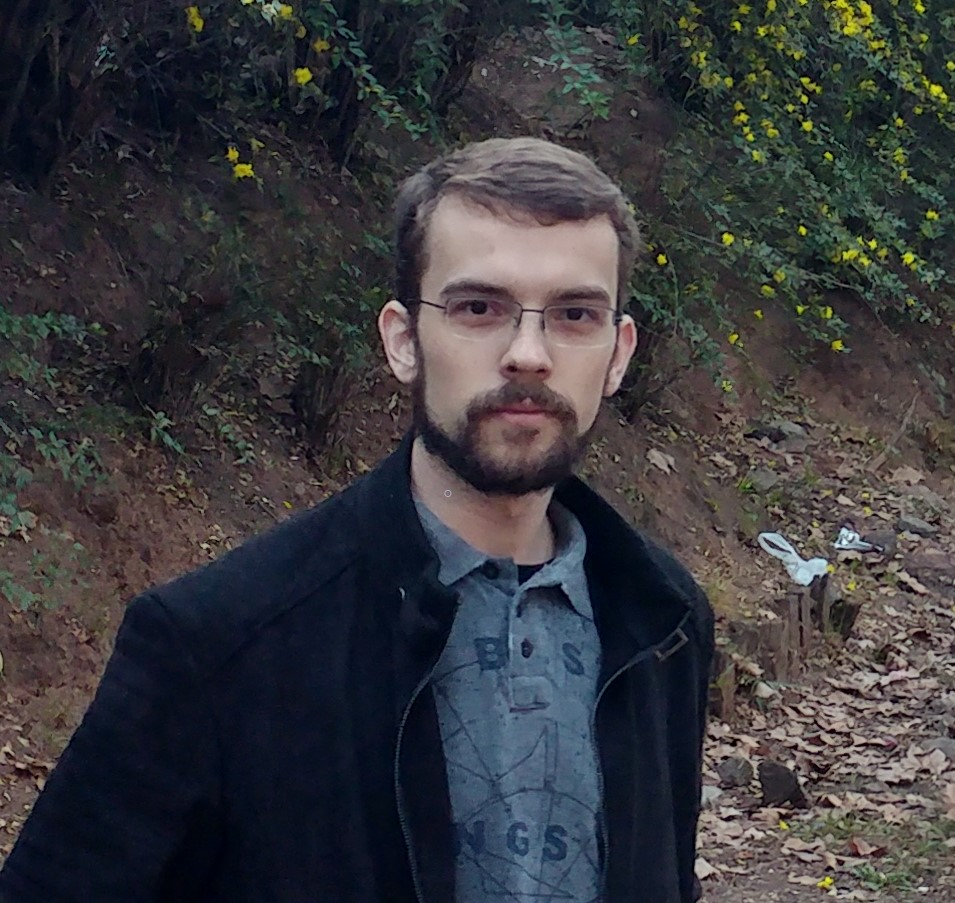
\includegraphics[width=1in,height=1.25in,clip,keepaspectratio]{riankoja}}]{Rian Koja}
% or if you just want to reserve a space for a photo:

%\begin{IEEEbiography}{Rian Koja}
Aerospace Engineer, Space Mechanics and Control Msc. Isolated discipline student at INPE.


\end{IEEEbiography}

\end{document}